\section{Coulomb-Nuclear Interference}
\label{sec:coulomb}

\TODO{Update this paragraph}.
This section presents a study of the measured differential cross-section focused on the effects of the Coulomb-nuclear interference (CNI). These effects are sensitive to the phase of nuclear amplitude and thus allow for determination of additional physics parameters such as $\rho$. The presentation starts with Section~\ref{sec:cni framework} outlining the theoretical concepts needed to describe the CNI effects. It is followed by Section~\ref{sec:cni task discussion} with a critical discussion on the task feasibility, presenting a strategy for the study. Section~\ref{sec:cni fit techniques} describes fit techniques used for parameter determination. As anticipated in the introduction, this study strongly benefits from including another high-statistics data set \cite{8tev-90m} obtained at the same energy however with beam optics $\beta^* = 90\un{m}$. This gives several possibilities of combination with the above presented data, from $\beta^* = 1000\un{m}$ optics. In particular, Section~\ref{sec:cni common fits} gives results where both data sets enter the fit on equal ground, while Section~\ref{sec:cni reciprocal fits} reports results where the data sets are assigned complementary roles.

\TODO{Which binning of 90m data is used}

\TODO{Move this paragraph after the framework section? It needs lots of terms defined there...}
\> define goals = by using data constrain nuclear amplitude:
\>> modulus -- non-exponentiality in nuclear component or CNI effect?
\>> phase -- value of $\rho$, test compatibility of central/peripheral phases, ...


%----------------------------------------------------------------------------------------------------

\subsection{Theoretical Framework}
\label{sec:cni framework}

In this section the different components of the combined elastic scattering cross-section, already briefly outlined in the introduction, are discussed in more detail. In particular, the Coulomb amplitude (Section~\ref{sec:cni coulomb}), the nuclear amplitude (Section~\ref{sec:cni nuclear}) and their interference (Section~\ref{sec:cni interference}).

\TODO{Expect three contributions to the amplitude, corresponding to Feynman diagram sets containing
\begin{itemize}
\item QED elements only -- calculable from first principles, Section~\ref{sec:cni coulomb}
\item QCD elements only -- not calculable from first principles, phenomenological amplitude used instead, Section~\ref{sec:cni nuclear}
\item both QED and QCD -- not calculable from first principles, phenomenological amplitude cannot be used either since this amplitude is correlated with the previous two. Section~\ref{sec:cni interference} will introduce two interference formulae attempting to calculate these effects.
\end{itemize}
}

%------------------------------------------------------------------
\subsubsection{Coulomb Amplitude}
\label{sec:cni coulomb}
%
The Coulomb amplitude can be calculated from QED (e.g.~Section 3.2 in \cite{block06}), using empirical electric ${\cal F}_{\rm E}$ and magnetic ${\cal F}_{\rm M}$ form factors of the proton. It can be shown (e.g.~Section 1.3.1 in~\cite{jan_thesis}) that, at low $|t|$, the effect of both form factors can be described by a single function ${\cal F}$:
\begin{equation}
\label{eq:coul cs}
	{\d\sigma^{\rm C}\over \d t} = {4\pi\alpha^2\over t^2}\,{\cal F}^4\ ,\qquad 
	{\cal F}^2 = {{\cal F}_{\rm E}^2 + \tau {\cal F}_{\rm M}^2\over 1 + \tau}\ ,\qquad 
	\tau = {|t|\over 4m^2}\ ,
\end{equation}
where $\alpha$ denotes the fine-structure constant and $m$ represents proton mass.

The form factors by Pucket et al.~\cite{puckett10} are used in this study and it will be shown that different choices have negligible impact on results presented later on.


%------------------------------------------------------------------
\subsubsection{Nuclear Amplitude}
\label{sec:cni nuclear}

Very few conclusions can be made on the nuclear amplitude from first principles (QCD). Instead, several phenomenology or theory motivated descriptions will be outlined here. The choice will be critically discussed in Section~\ref{sec:cni task discussion}.

%--------------------
\vskip3mm
\hbox to\hsize{\bf Modulus\hfil}

At $|t| \gtrsim 0.02\un{GeV^2}$ the effects due to the Coulomb interaction are not expected to be large (c.f.~Figure~\ref{fig:cni effect}). Thus, the measured cross-section can be -- to a large extent -- attributed to the nuclear component. Following Table~\ref{tab:data} and especially \cite{8tev-90m} which presents high-precision data for $|t| < 0.2\un{GeV^2}$, it is reasonable to parametrise the nuclear modulus as
\begin{equation}
\label{eq:nuc mod}
\left | {\cal A}^{\rm N}(t) \right | = \sqrt{s\over\pi} {p\over \hbar c} \sqrt{a} \exp\left( {1\over 2} \sum\limits_{n = 1}^{N_b} b_n\, t^n \right)\ ,
\end{equation}
where $N_b$ gives the number of free parameters in the exponent. This parametrisation is also compatible with a number of theoretical models (see e.g.~\cite{elegent}). \TODO{Consistently with \cite{8tev-90m}, $a$ gives differential cross-section intercept and $b_1$ forward diffractive slope}.

Since the calculation of Coulomb-nuclear interference may, in principle, involve integrations (e.g.~Eq.~(\ref{eq:int kl})), it is necessary to extend the parametrisation meaningfully to $|t| > 0.2\un{GeV^2}$. Therefore, at $|t| > 0.5\un{GeV^2}$, the parametrisation is anchored to a preliminary cross-section derived from the same data set as in \cite{8tev-90m} which features a dip-bump structure similar to the one observed at $\sqrt{s} = 7\un{TeV}$ \cite{epl95}. The region $0.2 < |t| < 0.5\un{GeV^2}$ is reserved for a smooth transition between the parametrisation in Eq.~(\ref{eq:nuc mod}) and the anchored part. It will be shown that changing the high-$|t|$ part has negligible impact on the results presented later on.


%--------------------
\vskip3mm
\hbox to\hsize{\bf Phase\hfil}

\TODO{$p_0$ always gives phase at $t=0$.}

\begin{figure*}
\begin{center}
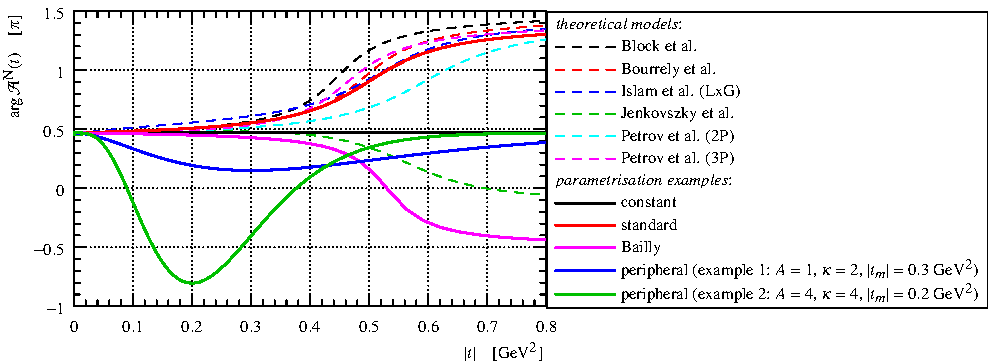
\includegraphics{fig/hadronic_phase_illustration.pdf}
\caption{Illustration of nuclear-phase forms. The dashed lines correspond to predictions by theoretical models (\cite{elegent} and references therein). The solid lines give typical examples of parametrisations used in the study, all at the same value of $\rho = 0.10$. The peripheral example corresponds to the central values in Eq.~(\ref{eq:nuc phase per val}).
}
\label{fig:phase illustration}
\end{center}
\end{figure*}


% ***
A {\it constant phase} is obviously the simplest choice:
\begin{equation}
\label{eq:nuc phase con}
\arg {\cal A}^{\rm N}(t) = p_0 = \hbox{const.}
\end{equation}
Note that this is equivalent to a strict proportionality of real and imaginary part of the amplitude at all $t$.

% ***
The {\it standard phase} parametrisation,
\begin{equation}
\label{eqn:nuc phase std}
\arg {\cal A}^{\rm N}(t) = p_{0} + \arctan \left(\frac{|t|-|t_{0}|}{\tau}\right) -  \arctan \left(\frac{-|t_{0}|}{\tau}\right) \: ,
\end{equation}
implements the main features of many theoretical models -- almost imaginary amplitude in the forward direction ($p_0 \approx \pi/2$) while almost purely real in the (first) diffraction dip. The parameters $t_0 = - 0.50\un{GeV^2}$ and $\tau = 0.1\un{GeV^2}$ have been chosen such that the shape is similar to a number of model predictions, see Figure~\ref{fig:phase illustration}.

% ***
Another parametrisation is by {\em Bailly et al.}~\cite{bailly87}:
\begin{equation}
\label{eq:nuc phase bai}
	%\arg {\cal A}^{\rm N}(t) = {\pi\over 2} - \arctan {\rho_0\over 1 - {t\over t_{\rm d}}},\ \rho_0 = {1\over \tan p_0}
	\arg {\cal A}^{\rm N}(t) = \arctan \left[ \tan p_0 \left(1 - {t\over t_{\rm d}} \right) \right]\ ,
\end{equation}
where $p_0$ determines the phase value at $t=0$ and $t_{\rm d} \approx -0.53\un{GeV^2}$ gives the position of the diffractive minimum at $8\un{TeV}$ (preliminary result derived from the $\beta^* = 90\un{m}$ data \cite{8tev-90m}). This phase has a behaviour qualitatively similar to the model of Jenskovszky et al., see Figure~\ref{fig:phase illustration}.

% ***
The {\it peripheral phase} \cite{kl94} provides an alternative to the above descriptions. As can be seen in Figure~\ref{fig:phase illustration}, the parametrisation
\begin{equation}
\label{eq:nuc phase per}
\arg {\cal A}^{\rm N}(t) = p_0 - \zeta_1 \left(- {t\over 1\un{GeV^2}} \right)^\kappa \e^{\nu t}
\end{equation}
can have rapid variation at low $|t|$, then peaks at $t = -\kappa / \nu$ and asymptotically returns to $p_0$, the value at $t=0$. According to \cite{kl-8tev}, the reasonable parameter values at $\sqrt s = 8\un{TeV}$ are
\begin{equation}
\label{eq:nuc phase per val}
	\zeta_1 = 800\ ,\qquad
	\kappa = 2.311 \pm 0.399\ ,\qquad
	\nu = (8.161 \pm 0.389)\un{GeV^{-2}}
\end{equation}
where the values after ``$\pm$'' indicate boundaries of ranges within which the values may be varied.


Figure~\ref{fig:phase illustration} presents a comparison of phase predictions of several models to typical examples of parametrisations proposed above.

It should be noted that the phase has decisive influence on the amplitude behaviour in the space of impact parameter, $b$, see e.g.~Section 3 in~\cite{klk02}. It can be characterised by the root-mean-squares (RMS) of $b$ for elastic and inelastic collisions. The constant, standard and Bailly phases lead to elastic collisions more central (smaller RMS) than the inelastic ones. The peripheral phase can yield a description with the opposite hierarchy, which is argued more natural by some authors (e.g. Section~4 in~\cite{kl96}). \TODO{Update: shape very relevant, too.}

%------------------------------------------------------------------
\subsubsection{Coulomb-Nuclear Interference Formulae}
\label{sec:cni interference}

The {\bf simplified West-Yennie formula (SWY)} \cite{wy68} is derived in the framework of perturbative quantum field theory by evaluating the lowest-order Feynman diagrams that comprise both nuclear and Coulomb interactions. In this approach, the interference is reduced to an additional phase between the Coulomb and nuclear amplitudes. Moreover, several approximations were used in the derivation. First, in order to avoid integrating over off-mass-shell contributions to the nuclear amplitude (poorly known), very slow variation of the nuclear amplitude phase was assumed: $\arg {\cal A}^{\rm N} \approx \hbox{const}$. Then, in order to obtain a closed-form expression, the exponential slope of the nuclear modulus
\begin{equation}
\label{eq:nuc slope}
B^{\rm N}(t) = {\d \log |{\cal A}^{\rm N}|^2 \over \d t}
\end{equation}
was assumed constant (i.e.~$b_2 = b_3 = 0$ in parametrisation Eq.~(\ref{eq:nuc mod})). The original formula did not contain the electromagnetic form factor ${\cal F}$, which was added later by hand:
\begin{equation}
\label{eq:int swy}
	{\d\sigma\over \d t}^{\rm C+N} = {\pi (\hbar c)^2 \over s p^2} \left | {\alpha s\over t} {\cal F}^2 \e^{\I\alpha \Phi(t)} + {\cal A}^{\rm N} \right |^2\ ,\qquad
	\Phi(t) = - \left( \log {B^{\rm N} |t|\over 2} + \gamma \right)\ ,
\end{equation}
where $\alpha$ is the fine-structure constant and $\gamma \doteq 0.577$ the Euler constant. Despite the many limitations, the formula has extensively been used in past data analyses. For backward-comparison reasons we consider it also in this report.

\begin{figure*}
\begin{center}
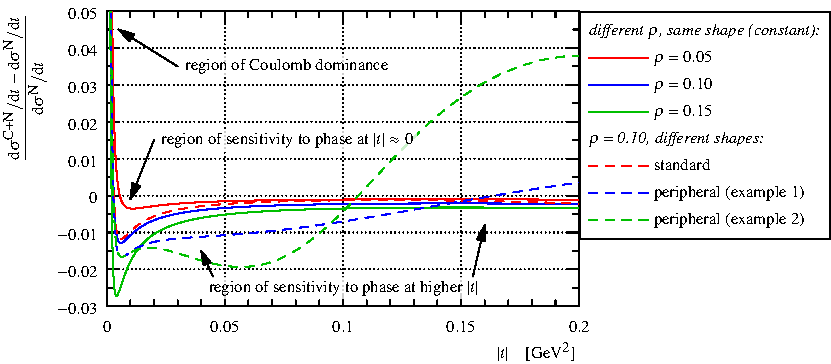
\includegraphics{fig/cni_effect_illustration.pdf}
\caption{%
Illustration of the effects due to the Coulomb interaction, using the KL formula. For the SWY formula, the picture is similar, however it misses the effects at higher $|t|$. The curves show a response of the interference formula to different nuclear phases with a purely exponential nuclear modulus. The solid curves correspond to phases of the same shape (constant) but different values of $\rho$: the maximal response can be seen at $|t| \lesssim 0.01\un{GeV^2}$. Conversely, the dashed lines correspond to phases with fixed $\rho$ but various shapes (the same examples as in Figure~\ref{fig:phase illustration}): response sizeable at $|t| \gtrsim 0.02\un{GeV^2}$.
}
\label{fig:cni effect}
\end{center}
\end{figure*}

The {\bf Kundr\' at-Lokaj\' i\v cek formula (KL)} \cite{kl94}\footnote{%
Note that many newer publications by the authors contain a misprint: wrong sign in front of the second term contributing to $G(t)$.
} was derived in an impact parameter formalism and it is based on the additivity of eikonals. The derivation poses no limitations on nuclear amplitude and the formula naturally incorporates the electromagnetic form factor. In this treatment, the interference effect goes beyond a single phase, the $G$ quantity is complex, in general:
\begin{equation}
\label{eq:int kl}
	\begin{aligned}
		{\d\sigma\over \d t}^{\rm C+N} &= {\pi (\hbar c)^2 \over s p^2} \left | {\alpha s\over t} {\cal F}^2
			+ {\cal A}^{\rm N}\, \Big[1 - \I\alpha G(t)\Big] \right |^2\ ,\cr
		G(t) &= 
			\int \d t'\, \log {t'\over t} {\d\phantom{t'}\over \d t'} {\cal F}^2(t')
			- \int \d t' \left( {{\cal A}^{\rm N}(t') \over {\cal A}^{\rm N}(t)} - 1 \right) { I(t, t')\over 2\pi }
			\ ,\cr
		I(t, t') &= \int_0^{2\pi} \d\phi\ {{\cal F}^2(t'')\over t''}\ ,\qquad t'' = t + t' + 2\sqrt{t\, t'} \cos\phi\ ,\cr
	\end{aligned}
\end{equation}
where the $t$ integrations go over the entire kinematically allowed region. A slightly different variant proposed in Eq.~(22) in~\cite{kl05} was considered, too:
\begin{equation}
\label{eq:int kl exp}
	{\d\sigma\over \d t}^{\rm C+N} = {\pi (\hbar c)^2 \over s p^2} \left | {\alpha s\over t} {\cal F}^2
		+ {\cal A}^{\rm N}\, \e^{- \I\alpha G(t)} \right |^2 \ .
\end{equation}

By analysing the formulae Eq.~(\ref{eq:int swy}) and (\ref{eq:int kl}), one can conclude that in the region where the nuclear amplitude dominates ($|t| \gtrsim 0.003\un{GeV^2}$), the effects due to the Coulomb interaction can be proportional either to $\alpha$ or to the ratio ${\cal A}^{\rm C} / {\cal A}^{\rm N}$. In both cases, the magnitude of the interference effects can be expected at a percent level, as shown in Figure~\ref{fig:cni effect}. The figure also shows that the effects at different $|t|$ probe different parts of the nuclear phase: maximum sensitivity to $\rho$ lies at very low $|t|$ while at higher $|t|$ the effects are sensitive to phase values at higher $|t|$. It can also be observed that for the constant, standard and Bailly phase the effects are very similar and rather mild at higher $|t|$. \TODO{Thus treat as one family}. This can be understood from a very limited variation of the phase at low $|t|$, which is the region contributing most to the integral in Eq.~(\ref{eq:int kl}). On the contrary, the higher $|t|$ response to peripheral phases can have various forms, often similar to the ``U shape'' of the reconstructed cross-section, see Figures~\ref{fig:fits common con} and~\ref{fig:fits common per}. \TODO{Recheck the statements about phase at ''higher $|t|$'' and correct if needed.}


%----------------------------------------------------------------------------------------------------
\subsection{Fitting Procedure}
\label{sec:fit}

Beyond using the data from Table~\ref{tab:data}, one might consider including $\beta^* = 90\un{m}$ data \cite{8tev-90m} which have much smaller uncertainties but reach limited to $|t| \gtrsim 0.03\un{GeV^2}$. Due to the latter, they have essentially no sensitivity to the $\rho$ parameter, cf.~Fig.~\ref{fig:cni effect}. Furthermore, due to possible systematic tensions between the data sets, including the $\beta^* = 90\un{m}$ data may have deteriorating impact on the $\rho$ determination. Therefore, the value of $\rho$ (or $p_0$ in other words), was determined from $\beta^* = 1000\un{m}$ data only. For other parameters to which both data sets have non-negligible sensitivity (e.g.~$b_i$ in Eq.~(\ref{eq:nuc mod})), both data sets shall give compatible results. This has been verified for all the fits presented later on. Since the $\beta^* = 90\un{m}$ data yield much lower uncertainties, both data sets have been used for determining all parameters except $\rho$. In practice, a series of two fits is performed:
\begin{enumerate}[leftmargin=2cm]
\item[step 1:] fit of $\beta^* = 1000\un{m}$ data with $p_0$ free,
\item[step 2:] fit of $\beta^* = 1000$ and $90\un{m}$ data with $p_0$ fixed from the preceding step.
\end{enumerate}

Each of the fits has been performed by following the standard least-squares method, however trying the following two implementations.

\begin{enumerate}

% ***
\item[A.] Minimise
\begin{equation}
\label{eq:chi sq A}
	\chi^2 = \Delta^\T \mat V^{-1} \Delta\ ,\qquad
	\Delta_i = \left.{\d\sigma\over \d t}\right|_{{\rm bin}\ i} - {\d\sigma^{\rm C+N}\over\d t}\left(t^{\rm rep}_{{\rm bin}\ i}\right)\ ,\qquad
	\mat V = \mat V_{\rm stat} + \mat V_{\rm syst} + \mat V_{\rm norm}\ ,
\end{equation}
where $\Delta$ is a vector of differences between the differential cross-section data and a fit function $\d\sigma^{C+N}/\d t$ evaluated at representative points $t^{\rm rep}$ of each bin \cite{lafferty94}. The minimisation is repeated several times and the representative points are updated between iterations. The covariance matrix $\mat V$ is composed of three components. The diagonal of $\mat V_{\rm stat}$ contains statistical uncertainty squared from Table~\ref{tab:data} and from Table~3 in \cite{8tev-90m}. $\mat V_{\rm syst}$ includes all systematic uncertainty contributions except normalisation, see Eq.~(\ref{eq:covar mat}) and Eq.~(14) in \cite{8tev-90m}. $\mat V_{\rm norm}$ reflects the normalisation uncertainty: $4.2\un{\%}$ fully correlated between the $90$ and $1000\un{m}$ datasets and $0.25\un{\%}$ ($0.08\un{\%}$) for $90\un{m}$ ($1000\un{m}$) dataset individually.


% ***
\item[B.] \TODO{Hubert's approach}
\begin{equation}
\label{eq:chi sq B}
	\chi^2 = \Delta^\T \mat V^{-1} \Delta + \TODO{...}\ ,\qquad
	\Delta_i = \left.{\d\sigma\over \d t}\right|_{{\rm bin}\ i} - {1\over \Delta t_i} \int_{{\rm bin}\ i} f(t)\,\d t\ ,\qquad
	\mat V = \mat V_{\rm stat} + \mat V_{\rm syst}\ ,
\end{equation}
$\Delta t_i$ representing the width of the $i$-th bin

\end{enumerate}

As anticipated above, one of the goals of this report is to probe the origin of the earlier observed differential cross-section non-exponentiality \cite{8tev-90m}. Therefore, the following two classes of fits will be considered.
\begin{itemize}
\item Section \ref{sec:fit exp1}: fits with purely-exponential nuclear modulus, that is $N_b=1$ in Eq.~(\ref{eq:nuc mod}). In this case, the non-exponentiality must come from the CNI effects.
\item Section \ref{sec:fit exp3}: fits with nuclear modulus flexible enough to describe the non-exponentiality with or without the CNI effects.
\end{itemize}


Three nuclear phase options have been considered which yield, as shown in Fig.~\ref{fig:bdist exp3}, three different levels of centrality/peripherality:
\begin{itemize}\setlength\itemsep{0pt}
\item constant phase, Eq.~(\ref{eq:nuc phase con}),
\item mid-peripheral phase, Eq.~(\ref{eq:nuc phase per}) with parameters free within the bounds in Eq.~(\ref{eq:nuc phase per val}),
\item full-peripheral phase, Eq.~(\ref{eq:nuc phase per}) with parameters fixed to the central values in Eq.~(\ref{eq:nuc phase per val}).
\end{itemize}

Below: brief description of attempts that have been tried but are not worth detailed discussion below.

\TODO{Tried several form-factors, no impact on the data.}

\TODO{Fits with constant, standard and Bailly phase practically indistinguishable $\rightarrow$ treated as one family represented by the constant phase.}

\TODO{Approaches A and B give compatible results $\rightarrow$ stability.}

\TODO{Fits with the two variants of the KL formula, Eqs.~(\ref{eq:int kl}) and (\ref{eq:int kl exp}), give compatible results.}

\TODO{Fits with different implementations of interference formulae (\cite{elegent} and custom) $\rightarrow$ confidence, no numerical issues.}



%----------------------------------------------------------------------------------------------------
\subsection{Fits with Purely-Exponential Nuclear Modulus}
\label{sec:fit exp1}

The goal of this section is to test whether the data are compatible with purely-exponential nuclear modulus, i.e.~$N_b=1$ in Eq.~(\ref{eq:nuc mod}). In other words, the non-exponetiality is forced come from the Coulomb-induced effects. For that two different nuclear phase options are considered: constant (as a representant of the central family), Eq.~(\ref{eq:nuc phase con}), and peripheral, Eq.~(\ref{eq:nuc phase per}), with parameters free within the ranges indicated in Eq.~(\ref{eq:nuc phase per val}). The fit results are summarised in Table~\ref{tab:fit exp1} and shown in Fig.~\ref{fig:fit exp1}.

\begin{table}
\caption{Fit results with $N_b=1$. Each column corresponds to a fit with different interference formula and/or nuclear phase. \TODO{add RMS of b?}}
\vskip-3mm
\label{tab:fit exp1}
\begin{center}
\setlength\tabcolsep{2.5mm}
\small
\input fig/fit_exp1/table_data.tex
\end{center}
\end{table}

\begin{figure*}
\begin{center}
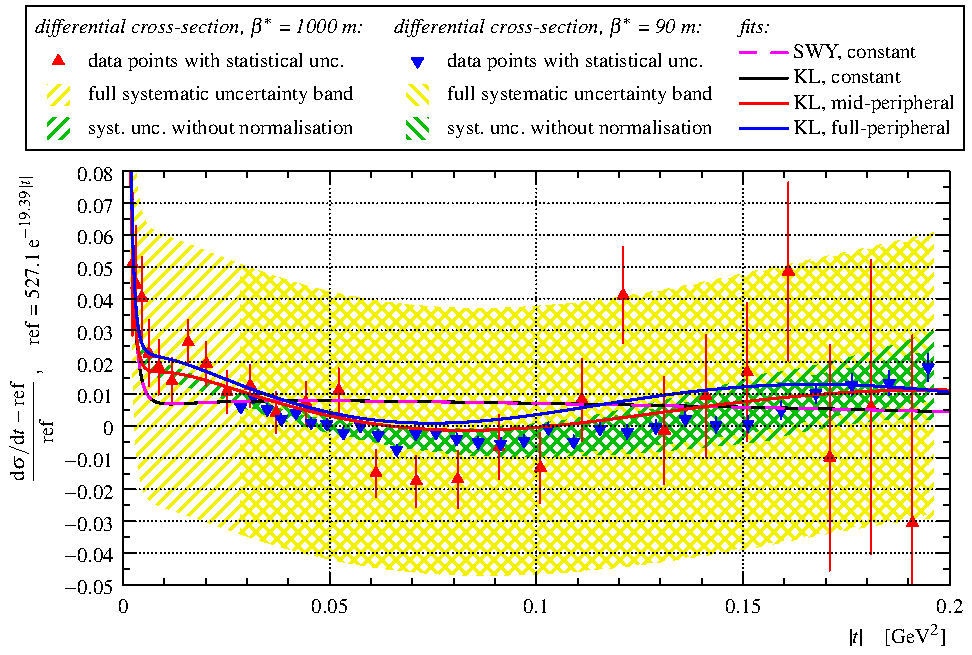
\includegraphics{fig/fit_exp1/t_dist_rel_with_fit.pdf}
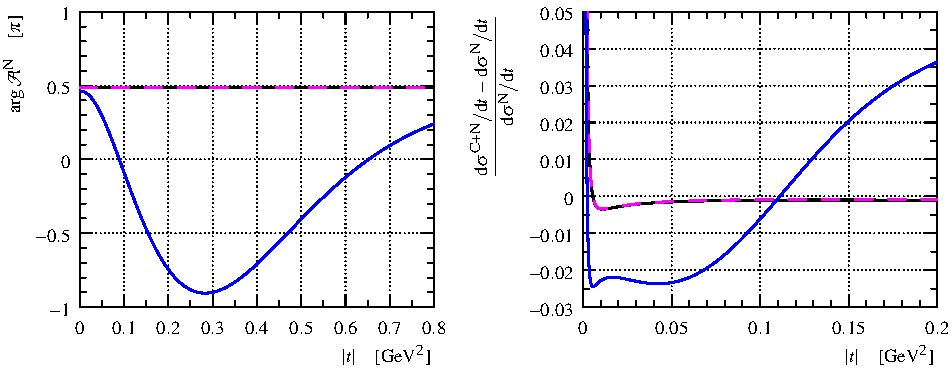
\includegraphics{fig/fit_exp1/phase_cni_effect.pdf}
\caption{Visualisation of fit results from Table~\ref{tab:fit exp1} obtained with $N_b=1$. The continuous (dashed) lines correspond to fits with KL (SWY) formula. Note that the fits with constant nuclear phase largely overlap.
TOP: fits compared to differential cross-section data in a relative reference frame, see the vertical axis label. The reference is identical to the one in \cite{8tev-90m}. 
BOTTOM LEFT: $t$-dependence of the nuclear phase as extracted from the fits.
BOTTOM RIGHT: the effects induced by the Coulomb interaction for each of the fits.
}%
\label{fig:fit exp1}
\end{center}
\end{figure*}

Table~\ref{tab:fit exp1} shows that both fits with constant phase are essentially identical and have bad fit quality. The step-2 fit using both $\beta^*=1000$ and $90\un{m}$ data can be excluded with $7.6\un{\sigma}$ significance. In turn, since the combination of $N_b=1$ and constant phase is the only compatible with the SWY formula, its use is excluded, too.

Although the quality of the fit with peripheral phases is good, but these options seem to be disfavoured from different perspectives.
\begin{itemize}
\item Most models predict non-exponential nuclear modulus, see e.g.~\cite{elegent}. Several reasons are summarised in \TODO{cite the KMR paper}.
\item The obtained value of $\rho$ is significantly lower than most extrapolations from lower energies \TODO{cite some of them}.
\item All the non-exponentiality is taken by CNI -- any special/extreme construction by Vojtech?? \TODO{formulate better.}
\end{itemize}


%----------------------------------------------------------------------------------------------------
\subsection{Fits with Non-Exponential Nuclear Modulus}
\label{sec:fit exp3}

The aim of this section is to discuss fits with enough flexibility in the nuclear modulus to describe the non-exponentiality in the data. For this, $N_b=2$ to $5$ were considered. The optimal degree was chosen according to two criteria: reasonable $\chi^2/\hbox{ndf}$ and stability of fit parameters (among which $\rho$ is one of the most sensitive). For example, with constant phase the fit (step 1) with $N_b=2$ yields $\chi^2/\hbox{ndf} = 1.07$ and $\rho = 0.101$ while with $N_b=3$ gives $\chi^2/\hbox{ndf} = 1.03$ and $\rho = 0.121$. Both fits have the normalised $\chi^2$ reasonably close to $1$, but the value of $\rho$ changes significantly between $N_b=2$ and $3$ which is unexpected should $N_b=2$ be sufficient. On the other hand $N_b=4$ gives $\chi^2/\hbox{ndf} = 0.861$ which is unreasonably low. Therefore $N_b=3$ was chosen.

The only applicable interference formula is KL.


\iffalse
* KL, exp2, con
\rh       =   0.101 \pm  0.026
last fit     : chi^2/ndf = 68.45/57 = 1.201, probability = 1.42E-01, significance = 1.467, quality = 0.000000
previous fit : chi^2/ndf = 27.74/26 = 1.067, probability = 3.71E-01, significance = 0.894

* KL, exp3, con
\rh       =   0.121 \pm  0.029
last fit     : chi^2/ndf = 57.59/56 = 1.028, probability = 4.16E-01, significance = 0.813, quality = 0.000000
previous fit : chi^2/ndf = 25.63/25 = 1.025, probability = 4.27E-01, significance = 0.794

* KL, exp4, con
rho    =   0.087 +-  0.034
last fit     : chi^2/ndf = 54.48/55 = 0.990, probability = 4.95E-01, significance = 0.683, quality = 0.000000
previous fit : chi^2/ndf = 20.66/24 = 0.861, probability = 6.59E-01, significance = 0.442
\fi


The fit with mid-peripheral phase has 7 free parameters ($\zeta_1$ is fixed) and varying many of them provokes similar changes in the cross-section shape. Therefore it is not surprising that several $\chi^2$ minima of similar quality can be found. In what follows, the minimum closest to the constant-fit will be reported.

As shown in Table~\ref{tab:fit exp3}, all the three fits yield very reasonable fit quality and remarkably comparable values of $\rho$ which are compared to previous measurements in Fig.~\ref{fig:rho cmp exp3}.

Fig.~\ref{fig:fit exp3} shows that the level of Coulomb-induced effects is different for the three fits. It is the mildest for the constant phase, more pronounced for the mid-peripheral and strongest for the full-peripheral. The same order can be observed in the variation of the nuclear phase as function of $|t|$.

The impact-parameter distribution \TODO{ref} for the three fits is shown in Fig.~\ref{fig:bdist exp3}, also giving the RMS for elastic, inelastic and total collisions \TODO{ref}. The fit with constant phase exhibits central behaviour: the elastic impact-parameter distribution is peaked at $b=0$ and the elastic RMS is smaller than the inelastic one. The mid-peripheral fit corresponds to the case where all three RMS values are comparable. The full-peripheral fit has truly peripheral behaviour: the distribution maximum lies at $b > 0$ and the elastic RMS is grater that the inelastic.

\TODO{Statement about si tot: stability (also wrt. Nb=1) and that compatible but little higher (as expected) compared to the previous results.}

\begin{table}
\caption{Fit results with KL formula and $N_b=3$. \TODO{add RMS of b?}}
\vskip-3mm
\label{tab:fit exp3}
\begin{center}
\setlength\tabcolsep{5mm}
\small
\input fig/fit_exp3/table_data.tex
\end{center}
\end{table}

\begin{figure*}
\begin{center}
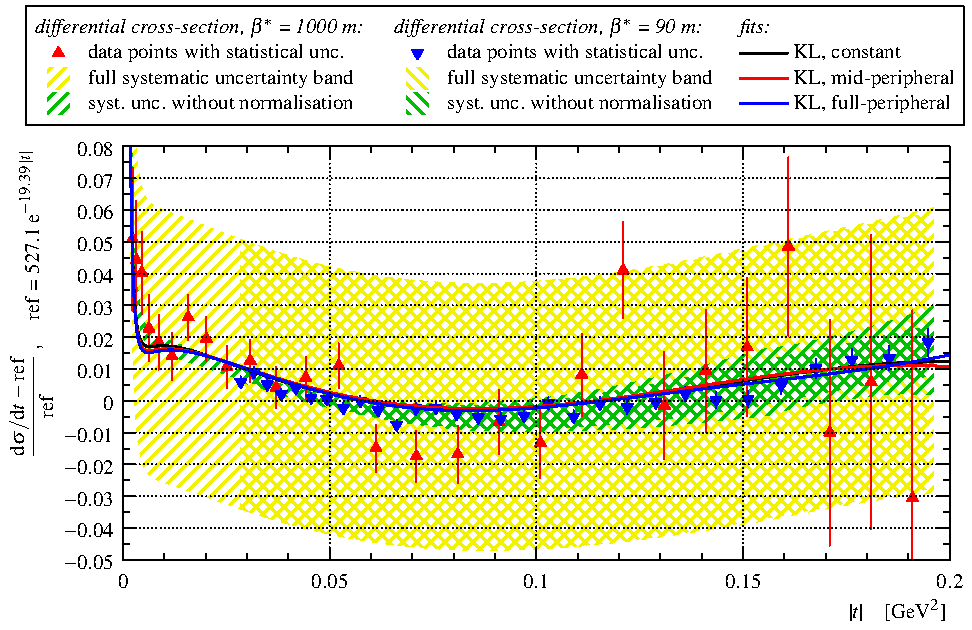
\includegraphics{fig/fit_exp3/t_dist_rel_with_fit.pdf}
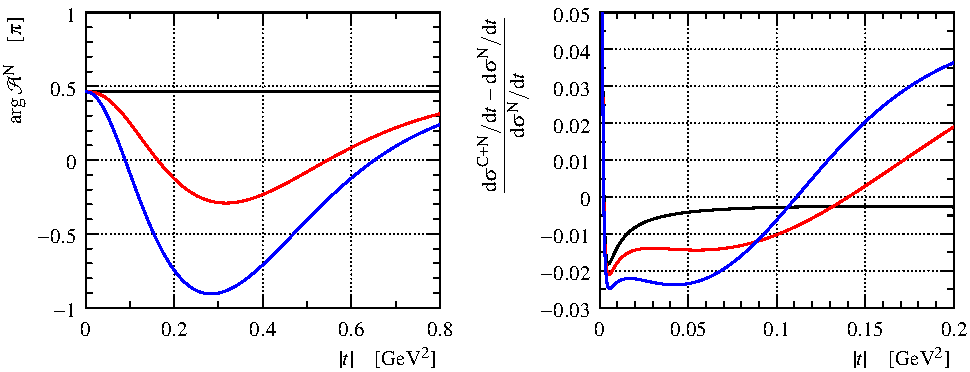
\includegraphics{fig/fit_exp3/phase_cni_effect.pdf}
\caption{Visualisation of fit results from Table~\ref{tab:fit exp3} obtained with KL formula and $N_b=3$. The solid lines correspond to fits with different nuclear phases.
TOP: fits compared to differential cross-section data in a relative reference frame, see the vertical axis label. The reference is identical to the one in \cite{8tev-90m}. 
BOTTOM LEFT: $t$-dependence of the nuclear phase as extracted from the fits.
BOTTOM RIGHT: the effects induced by the Coulomb interaction for each of the fits.
}%
\label{fig:fit exp3}
\end{center}
\end{figure*}

\begin{figure*}
\begin{center}
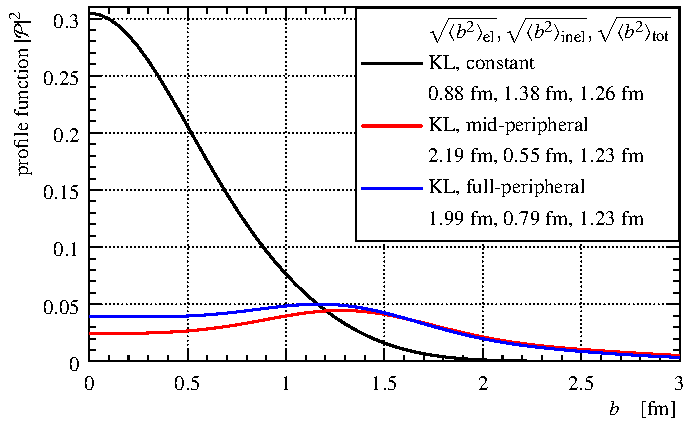
\includegraphics{fig/fit_exp3/b_dist.pdf}
\caption{TODO
}%
\label{fig:bdist exp3}
\end{center}
\end{figure*}


\begin{figure*}
\begin{center}
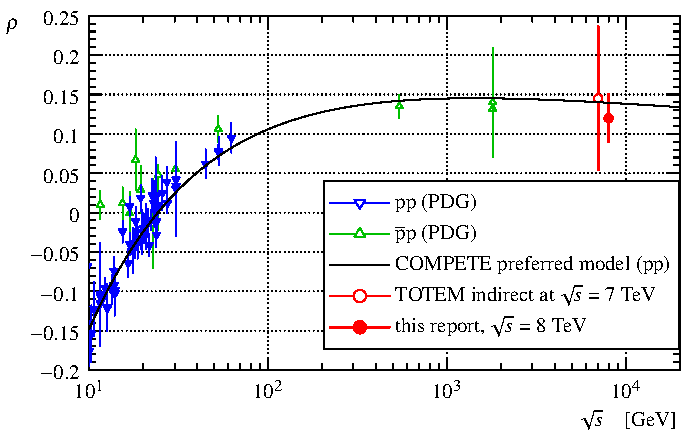
\includegraphics{fig/rho_s.pdf}
\caption{Energy dependence of the $\rho$ parameter. The blue (green) hollow triangles correspond to $\rm pp$ ($\rm \bar pp$) data from PDG \cite{pdg} \TODO{warning: most of points likely to be determined by SWY}. The hollow red dot stands for the earlier indirect determination by TOTEM \cite{epl101-tot}. The full red dot represents the three results from Table~\ref{tab:fit exp3} which happen to be identical within the resolution. The black curve gives the preferred $\rm pp$ model by COMPETE \cite{compete}, obtained without using LHC data.
}%
\label{fig:rho cmp exp3}
\end{center}
\end{figure*}
